\section{\large \textcolor{blue}{As leis da Termodinâmica}}

\begin{flushleft}
\textbf{\textcolor{blue}{\Large Quest\~ao - IFSP 2015 - Lei de Fourier da Condu\c{c}\~ao de Calor}}\\
\noindent

\subsection{Quest\~ao IFSP 2015 - Lei de Fourier da Condu\c{c}\~ao de Calor}

Em um experimento sobre condutividade térmica dos metais, uma barra metálica homogênea e de área de secção transversal uniforme, isolada termicamente do meio externo, foi colocada entre duas fontes a temperaturas diferentes ($T_A$ e $T_B$). Dois termômetros foram colocados de forma a medirem a temperatura da barra em dois pontos diferentes e estabilizaram seus valores naqueles mostrados na figura abaixo.

\vspace{0.3cm}

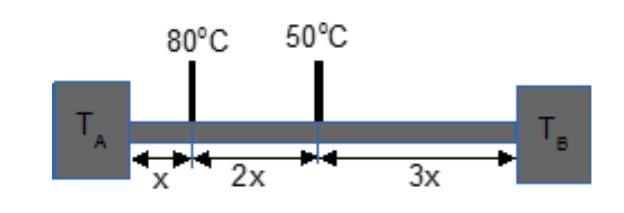
\includegraphics[width=0.8\textwidth]{figures/barra_termica.png}

\vspace{0.3cm}

A temperatura das fontes ($T_A$ e $T_B$) são, respectivamente:

\begin{itemize}
\item[(A)] 90\textdegree C e 20\textdegree C
\item[(B)] 125\textdegree C e 5\textdegree C
\item[(C)] 120\textdegree C e 16,6\textdegree C
\item[(D)] 95\textdegree C e 5\textdegree C
\item[(E)] 20\textdegree C e 90\textdegree C
\end{itemize}

\vspace{0.5cm}

\textcolor{red}{\textbf{Solução:}}\\

Como a barra é homogênea, de área constante e está isolada termicamente, o sistema está em equilíbrio térmico e o fluxo de calor é constante. A distribuição de temperatura é linear em cada trecho. Assim, podemos aplicar a relação:

\[
\frac{\Delta T_1}{L_1} = \frac{\Delta T_2}{L_2} = \frac{\Delta T_3}{L_3}
\]

Dividindo a barra em 3 trechos:
\begin{itemize}
\item Do ponto $T_A$ até 80\textdegree C: comprimento $x$, variação de temperatura: $T_A - 80$
\item De 80\textdegree C até 50\textdegree C: comprimento $2x$, variação de temperatura: $30$
\item De 50\textdegree C até $T_B$: comprimento $3x$, variação de temperatura: $50 - T_B$
\end{itemize}

Igualando as razões:

\[
\frac{T_A - 80}{x} = \frac{30}{2x} \Rightarrow T_A - 80 = 15 \Rightarrow T_A = 95^\circ \text{C}
\]

\[
\frac{30}{2x} = \frac{50 - T_B}{3x} \Rightarrow 15 = \frac{50 - T_B}{3} \Rightarrow 50 - T_B = 45 \Rightarrow T_B = 5^\circ \text{C}
\]

\vspace{0.3cm}

A resposta correta é a alternativa \colorbox{green!50}{\textbf{(D)}}.

\end{flushleft}


\begin{flushleft}
\textbf{\textcolor{blue}{\Large Quest\~ao 34 - IFSP 2017 - Entropia}}\\
\noindent

\subsection{Quest\~ao 34 - IFSP 2017 - Entropia}
Dois corpos de diferentes materiais e temperaturas s\~ao colocados em uma caixa termicamente isolada. 
O material 1, com 200 g e temperatura de 40\textdegree C, possui $c_1 = 300 \, \text{J/kg.K}$; e o material 2, 
com 100 g e temperatura de 100\textdegree C, possui $c_2 = 120 \, \text{J/kg.K}$. Qual a varia\c{c}\~ao de entropia do 
sistema ap\'os atingir o equil\'ibrio t\'ermico?

\begin{itemize}
\item[(A)] -0,16 J/K
\item[(B)] 0,16 J/K
\item[(C)] 5,07 J/K
\item[(D)] 72,31 J/K
\end{itemize}

\vspace{0.5cm}

\textcolor{red}{\textbf{Solução:}}\\

Como o sistema é termicamente isolado, usamos a conserva\c{c}\~ao da energia para encontrar a temperatura final de equil\'ibrio $T_f$:

\[
m_1 c_1 (T_f - T_1) + m_2 c_2 (T_f - T_2) = 0
\]

\[
0{,}2 \cdot 300 \cdot (T_f - 313{,}15) + 0{,}1 \cdot 120 \cdot (T_f - 373{,}15) = 0
\Rightarrow T_f = 323{,}15\, \text{K}
\]

A varia\c{c}\~ao de entropia total do sistema ser\'a:

\[
\Delta S = m_1 c_1 \ln \left( \frac{T_f}{T_1} \right) + m_2 c_2 \ln \left( \frac{T_f}{T_2} \right)
\]

\[
\Delta S = 0{,}2 \cdot 300 \cdot \ln\left( \frac{323{,}15}{313{,}15} \right) + 0{,}1 \cdot 120 \cdot \ln\left( \frac{323{,}15}{373{,}15} \right)
\]

\[
\Delta S \approx 60 \cdot 0{,}0314 + 12 \cdot (-0{,}1437) \approx 1{,}884 - 1{,}724 = \boxed{0{,}16 \, \text{J/K}}
\]

A resposta correta é alternativa \colorbox{green!50}{\textbf{B}}.

\end{flushleft}

\section*{Ciclos Termodinâmicos — Descrição Detalhada}

\subsection*{O que é um ciclo termodinâmico?}

Um \colorbox{yellow!40}{\textbf{ciclo termodinâmico} é uma sequência de processos termodinâmicos} realizados por um sistema (geralmente um fluido de trabalho), que retorna ao seu estado inicial ao final do ciclo.

O sistema troca calor \(Q\) com o meio externo e realiza trabalho \(W\), obedecendo à Primeira Lei da Termodinâmica:
\[
\Delta U = Q - W
\]

Como o \colorbox{yellow!40}{sistema retorna ao estado inicial (\(\Delta U = 0\))}, temos:
\[
Q_{\text{líquido}} = W_{\text{líquido}}
\]

\begin{itemize}
  \item Se \colorbox{yellow!40}{o ciclo for \textbf{motor}: transforma calor em trabalho (\(W_{\text{líquido}} > 0\)).}
  \item Se for \textbf{refrigerador/bomba de calor}: consome trabalho para transferir calor de um reservatório frio para um quente.
\end{itemize}

\subsection*{Ciclos Motores (Máquinas Térmicas)}

\subsubsection*{\colorbox{yellow!40}{Ciclo de Carnot}}

Ciclo ideal com a máxima eficiência possível entre duas temperaturas \(T_q\) (quente) e \(T_f\) (fria).

\begin{enumerate}
  \item \colorbox{green!30}{Isotérmica a \(T_q\) (expansão com entrada de calor \(Q_q\))}
  \item \colorbox{green!30}{Adiabática (expansão até \(T_f\))}
  \item \colorbox{green!30}{Isotérmica a \(T_f\) (compressão com rejeição de calor \(Q_f\))}
  \item \colorbox{green!30}{Adiabática (compressão até \(T_q\))}
\end{enumerate}

Eficiência ideal:
\[
\boxed{
\eta_C = 1 - \frac{T_f}{T_q}
}
\]

\section*{O Ciclo de Carnot é Irreversível?}

\textbf{Resposta curta:} \textbf{Não. O ciclo de Carnot é, por definição, completamente reversível.}

\subsection*{Por quê?}

O ciclo de Carnot é um modelo teórico ideal que estabelece o limite máximo de eficiência entre duas temperaturas \( T_q \) (quente) e \( T_f \) (fria). Ele é composto por quatro transformações \textbf{reversíveis}:
\begin{itemize}
  \item Duas isotérmicas reversíveis:
    \begin{itemize}
      \item Expansão isotérmica a \( T_q \) (absorve calor \( Q_q \))
      \item Compressão isotérmica a \( T_f \) (rejeita calor \( Q_f \))
    \end{itemize}
  \item Duas adiabáticas reversíveis:
    \begin{itemize}
      \item Expansão adiabática (sem troca de calor)
      \item Compressão adiabática (sem troca de calor)
    \end{itemize}
\end{itemize}

Cada processo ocorre de modo infinitamente lento, mantendo o sistema em equilíbrio e sem produção de entropia:
\[
\oint \frac{\delta Q}{T} = 0
\]

\subsection*{Na prática}

Nenhuma máquina real pode executar um ciclo de Carnot, pois:
\begin{itemize}
  \item As trocas infinitesimais de calor requerem tempo infinito.
  \item Sempre há atrito, dissipação e gradientes de temperatura.
\end{itemize}

Portanto:
\begin{center}

\textbf{Ciclo de Carnot ideal: reversível e eficiência máxima.}\\
\textbf{Máquinas reais: irreversíveis e menos eficientes.}
\end{center}

\begin{table}[h!]
\centering
\small
\caption{Comparação entre o Ciclo de Carnot e Ciclo Real}
\begin{tabular}{|c|c|c|}
\hline
\textbf{Característica} & \textbf{Ciclo de Carnot (Ideal)} & \textbf{Ciclo Real} \\ \hline
\textbf{Reversibilidade} 
& Totalmente reversível & Irreversível (perdas) \\ \hline
\textbf{Produção/entropia} 
& Zero & Maior que zero \\ \hline
\textbf{Eficiência} 
& Máxima teórica & Menor que Carnot \\ \hline
\textbf{Processos} 
& Isotérmicos/adiabáticos & Processos com dissipação\\ \hline
\textbf{Velocidade/operação} 
& Infinitamente lenta & Finita \\ \hline
\textbf{Aplicabilidade} 
& Apenas modelo teórico & Realizado em motores/máquinas \\ \hline
\end{tabular}
\end{table}


\subsubsection*{Ciclo Otto}

Modelo ideal para motores a gasolina (ignição por centelha).

\begin{enumerate}
  \item Compressão adiabática
  \item Aquecimento a volume constante (explosão da mistura combustível-ar)
  \item Expansão adiabática
  \item Resfriamento a volume constante (descarga dos gases)
\end{enumerate}

Eficiência ideal:
\[
\eta_O = 1 - \frac{1}{r^{\gamma-1}}, \quad r = \frac{V_{\text{máx}}}{V_{\text{mín}}}, \quad \gamma = \frac{c_p}{c_v}
\]

\subsubsection*{Ciclo Diesel}

Modelo para motores diesel (ignição por compressão). Difere do Otto: calor adicionado a pressão constante.

\begin{enumerate}
  \item Compressão adiabática
  \item Aquecimento a pressão constante
  \item Expansão adiabática
  \item Resfriamento a volume constante
\end{enumerate}

\subsubsection*{Ciclo de Brayton (ou Joule)}

Usado em turbinas a gás e motores a jato.

\begin{enumerate}
  \item Compressão adiabática
  \item Aquecimento a pressão constante
  \item Expansão adiabática
  \item Resfriamento a pressão constante
\end{enumerate}

\subsection*{Ciclos de Refrigeração e Bombas de Calor}

\subsubsection*{Ciclo inverso de Carnot}

Mesmo princípio do Carnot, mas “ao contrário”. Usa trabalho para transferir calor de \(T_f\) para \(T_q\).

Coeficiente de performance (COP):
\begin{itemize}
  \item Refrigerador: 
  \[
  COP_R = \frac{T_f}{T_q - T_f}
  \]
  \item Bomba de calor: 
  \[
  COP_B = \frac{T_q}{T_q - T_f}
  \]
\end{itemize}

\subsubsection*{Ciclo de Compressão de Vapor}

Usado em geladeiras e ar-condicionado.

\begin{enumerate}
  \item Compressão adiabática (fluido é comprimido e aquecido)
  \item Condensação a pressão constante (rejeita calor para o ambiente)
  \item Expansão isentrópica (queda de \(P\) e \(T\))
  \item Vaporização a pressão constante (absorve calor do ambiente interno)
\end{enumerate}

\subsection*{Resumo das Grandezas Importantes}

Eficiência térmica de uma máquina térmica:
\[
\eta = \frac{W_{\text{líquido}}}{Q_{\text{quente}}}
\]

COP para refrigeradores e bombas:
\begin{itemize}
  \item Refrigerador: \(COP_R = \frac{Q_f}{W}\)
  \item Bomba de calor: \(COP_B = \frac{Q_q}{W}\)
\end{itemize}

\subsection*{Observação Prática}

\begin{itemize}
  \item \colorbox{green!30}{Ciclos reais sempre têm perdas por atrito, irreversibilidades} e transferência de calor fora do equilíbrio — por isso a eficiência real é menor que a teórica.
  \item O \colorbox{green!30}{\textbf{Ciclo de Carnot} é um limite superior (ideal), mas impraticável na prática.}
\end{itemize}

\begin{flushleft}
\textbf{\textcolor{blue}{\Large Quest\~ao - 39 IFSC 2023 - Ciclos Termodinamicos - Diesel}}\\
\noindent

\subsection{Quest\~ao - 39 IFSC 2023 - Ciclos Termodinamicos - Diesel}

Os ciclos termodin\^amicos s\~ao fen\^omenos que envolvem a convers\~ao de energia t\'ermica em trabalho mec\^anico ou a 
realiza\c{c}\~ao de trabalho mec\^anico em um sistema. Esses ciclos abrangem uma variedade de configura\c{c}\~oes e t\^em 
aplica\c{c}\~oes em diversos campos. Um exemplo relevante \'e o ciclo Diesel, amplamente utilizado em motores de combust\~ao 
interna. Com base no exposto acima e considerando o ciclo Diesel te\'orico apresentado no gr\'afico da Figura 3 abaixo, 
relacione a Coluna 1 \`a Coluna 2.

\begin{center}
\centering
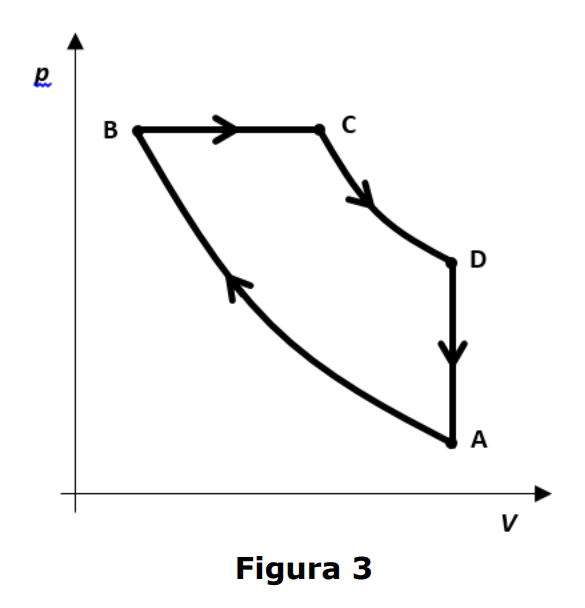
\includegraphics[scale=0.5]{figures/ciclo-termodinamico-diesel.png}
\end{center}

\bigskip

\noindent
\textbf{Coluna 1}
\begin{enumerate}
\item Curva A$\to$B
\item Curva B$\to$C
\item Curva C$\to$D
\item Curva D$\to$A
\end{enumerate}

\noindent
\textbf{Coluna 2}
\begin{itemize}
\item[(\ )] Realiza\c{c}\~ao de trabalho pelo sistema.
\item[(\ )] Transformação adiabática.
\item[(\ )] Rejei\c{c}\~ao de calor pelo sistema.
\item[(\ )] Realiza\c{c}\~ao de trabalho pelo sistema.
\end{itemize}

A ordem correta de preenchimento dos par\^enteses, de cima para baixo, \'e:

\begin{itemize}
\item[(A)] 2 -- 1 -- 4 -- 3.
\item[(B)] 3 -- 2 -- 4 -- 1.
\item[(C)] 2 -- 4 -- 1 -- 3.
\item[(D)] 3 -- 2 -- 4 -- 1.
\item[(E)] 2 -- 4 -- 2 -- 3.
\end{itemize}

\vspace{0.5cm}

\textcolor{red}{\textbf{Solução:}}\\

\textbf{Observação preliminar:} No ciclo Diesel teórico (representado no diagrama $p\times V$), as quatro transformações usuais s\~ao:
\begin{itemize}
    \item compress\~ao adiab\'atica (estado inicial $\to$ estado comprimido),
    \item aquecimento a press\~ao quase constante (adi\c{c}\~ao de calor isob\'arica),
    \item expans\~ao adiab\'atica (realiza trabalho),
    \item rejei\c{c}\~ao de calor em volume praticamente constante (isoqu\'arico/isochorico).
\end{itemize}

Agora analisamos cada curva do enunciado com base no diagrama:

\begin{enumerate}
    \item \textbf{Curva A$\to$B:} No diagrama, A est\'a em uma posi\c{c}\~ao com maior volume e menor press\~ao; ao ir para B a press\~ao aumenta e o volume diminui — trata-se de compress\~ao sem trocas de calor (adiab\'atica ideal). Portanto \textbf{A$\to$B = transforma\c{c}\~ao adiab\'atica}. (corresponde ao item \emph{Transformação adiabática}).
    \item \textbf{Curva B$\to$C:} Apresenta press\~ao aproximadamente constante enquanto o volume aumenta (seta para a direita) — caracteriza adi\c{c}\~ao de calor a press\~ao constante com expans\~ao: o sistema \textbf{realiza trabalho} sobre o meio externo. (corresponde a \emph{Realização de trabalho pelo sistema}).
    \item \textbf{Curva C$\to$D:} \'E uma expans\~ao onde a press\~ao e o volume variam com forma curva (queda de press\~ao com aumento de volume) — 
    corresponde \`a \textbf{expans\~ao adiab\'atica} (o sistema tamb\'em realiza trabalho nessa etapa). (corresponde a \emph{Realização de trabalho pelo sistema}).
    \item \textbf{Curva D$\to$A:} Apresenta varia\c{c}\~ao de press\~ao a volume praticamente constante (seta vertical) — corresponde \`a \textbf{rejei\c{c}\~ao de calor} (isoqu\'arica/isoch\'orica) que leva o sistema de volta ao estado inicial. (corresponde a \emph{Rejeição de calor pelo sistema}).
\end{enumerate}

Associando as curvas (n\'umero da Coluna 1) \`a descri\c{c}\~ao da Coluna 2 (de cima para baixo):

\begin{itemize}
    \item Realiza\c{c}\~ao de trabalho pelo sistema. \quad $\to$ Curva \textbf{2} (B$\to$C).
    \item Transformação adiabática. \quad\quad\quad\quad\ \ $\to$ Curva \textbf{1} (A$\to$B).
    \item Rejeição de calor pelo sistema. \quad\quad\ $\to$ Curva \textbf{4} (D$\to$A).
    \item Realiza\c{c}\~ao de trabalho pelo sistema. \quad $\to$ Curva \textbf{3} (C$\to$D).
\end{itemize}

Logo, a sequ\^encia \emph{de cima para baixo} \'e \(\;2\;-\;1\;-\;4\;-\;3\;\).

\vspace{0.3cm}

\textbf{Resposta:} \colorbox{green!50}{\textbf{A}}.

\end{flushleft}

\begin{flushleft}
\textbf{\textcolor{blue}{\Large Quest\~ao 40 - Termodinâmica: Funções de Estado}}\\
\noindent
\subsection{Quest\~ao 40 - IFS 2024 Termodinâmica: Funções de Estado}
Uma função de estado de um sistema termodinâmico fica
completamente definida quando o estado do sistema é
especificado. Isso pode ser representado num diagrama
pressão-volume do sistema, que ilustra seus estados inicial
e final. Qual das grandezas abaixo é uma função de estado
de um sistema termodinâmico?

\begin{itemize}
\item[(A)] A energia interna.
\item[(B)] O calor.
\item[(C)] O trabalho.
\item[(D)] A massa.
\end{itemize}

\vspace{0.5cm}

\textcolor{red}{\textbf{Solução:}}\\

\section*{Introdução: Funções de Estado em Termodinâmica}

A Termodinâmica é a área da Física que estuda as transformações de energia e as propriedades macroscópicas da matéria, como temperatura, pressão e volume. Para descrever um sistema termodinâmico, é necessário especificar o \textbf{estado do sistema}, que é determinado por um conjunto de variáveis chamadas \textbf{variáveis de estado}.

Quando um sistema evolui de um estado inicial para um estado final, podemos calcular as mudanças sofridas em algumas grandezas físicas. Algumas dessas grandezas dependem apenas do estado inicial e final do sistema, enquanto outras dependem do caminho seguido durante o processo.

\subsection*{O que é uma função de estado?}

Uma \textbf{função de estado} é uma grandeza física cujo valor só depende do estado atual do sistema, isto é, das condições termodinâmicas (como \(P\), \(V\), \(T\), \(U\) etc.), e \textbf{não depende do processo pelo qual o sistema chegou a esse estado}.

Ou seja:
\begin{quote}
As funções de estado são propriedades macroscópicas que caracterizam completamente o estado do sistema. Sua variação entre dois estados é a mesma, independentemente do caminho percorrido entre eles.
\end{quote}

\subsection*{Exemplos clássicos de funções de estado:}
\begin{itemize}
    \item Energia interna (\(U\))
    \item Entalpia (\(H\))
    \item Entropia (\(S\))
    \item Pressão (\(P\))
    \item Volume (\(V\))
    \item Temperatura (\(T\))
\end{itemize}

Essas grandezas podem ser representadas em diagramas, como os famosos diagramas \(P \times V\) ou \(T \times S\), que ilustram estados e trajetórias de processos.

\subsection*{E o que não é função de estado?}

Grandezas como o \textbf{calor trocado} (\(Q\)) e o \textbf{trabalho realizado} (\(W\)) durante um processo dependem de 
como o sistema evoluiu — são chamadas de \textbf{funções de processo}.

Por exemplo: para comprimir um gás do volume \(V_1\) ao volume \(V_2\), o trabalho realizado pode ser maior ou menor 
dependendo do caminho seguido (isotérmico, adiabático etc.), mas a variação de energia interna só depende do estado inicial e final.

A resposta correta é alternativa \colorbox{green!50}{\textbf{A}}.
\end{flushleft}

\noindent\rule{\linewidth}{0.6pt}\\

\begin{flushleft}
\textbf{\textcolor{blue}{\Large Quest\~ao 41 - Lei da Termodinâmica: Carnot}}\\
\noindent
\subsection{Quest\~ao 41 - Lei da Termodinâmica: Carnot}
Uma bomba de calor serve para extrair calor do ambiente
externo a 7°C e aquecer o interior de uma casa a 27°C.
Considerando que a bomba é uma máquina de Carnot, para
cada 15.000 J de calor entregue dentro de casa, a menor
quantidade de trabalho que deve ser fornecido à bomba é

\begin{itemize}
\item[(A)] 2.500 J.
\item[(B)] 2.000 J.
\item[(C)] 1.500 J.
\item[(D)] 1.000 J.
\end{itemize}

\vspace{0.5cm}

\textcolor{red}{\textbf{Solução:}}\\

\section*{Definição}

Uma máquina térmica converte calor em trabalho, operando entre duas fontes térmicas.

\section*{Rendimento}

\[
\eta = \frac{W}{Q_q} = \frac{Q_q - Q_f}{Q_q} = 1 - \frac{Q_f}{Q_q}
\]

\begin{itemize}
  \item \( \eta \): rendimento
  \item \( W \): trabalho útil
  \item \( Q_q \): calor absorvido da fonte quente
  \item \( Q_f \): calor rejeitado à fonte fria
\end{itemize}

\section*{Rendimento da Máquina de Carnot}

\[
\eta_{\text{Carnot}} = 1 - \frac{T_f}{T_q}
\]

\subsection*{Calcular o rendimento da bomba de calor:}

\[
\eta = 1 - \frac{T_f}{T_q} = 1 - \frac{7^{\circ}\textrm{C} + 273\textrm{K}}{27^{\circ}\textrm{C}+ 273\textrm{K}} = 1 - \frac{280}{300} = 1 - 0.933333 = 0.066667 = 6.67\%
\]

Agora podemos calcular o trabalho realizado pela bomba de calor:

\[
  W = \eta Q_q = 6.67\% \times 15.000 \textrm{J} = 1.000 \textrm{J}
\]
A resposta correta é alternativa \colorbox{green!50}{\textbf{D}}.
\end{flushleft}

\noindent\rule{\linewidth}{0.6pt}\\

\section*{Princ\'ipios da Termodinâmica}

\subsection*{Primeiro Princípio}
\begin{equation*}
    \Delta U = Q - W   \hspace{0.5cm} \longrightarrow \hspace{0.5cm} Q = W + \Delta U
\end{equation*}
\subsection*{Segundo Princípio}
\begin{itemize}
    \item O calor não flui espontaneamente de um corpo frio para um corpo quente.
    \item Entropia tende a aumentar.
\end{itemize}

\section*{O que é entropia?}
A entropia (\(S\)) é uma função de estado que mede o grau de desordem de um sistema, a quantidade de microestados possíveis, e a irreversibilidade de processos.

\section*{Definição termodinâmica}
Para processos reversíveis:

\[
\Delta S = \int \frac{dQ_{\text{rev}}}{T}
\]

Para temperatura constante (isotérmico):

\[
\Delta S = \frac{Q_{\text{rev}}}{T}
\]

\section*{Segunda Lei da Termodinâmica}

\[
\Delta S_{\text{total}} \geq 0
\]

\begin{itemize}
  \item \( \Delta S_{\text{total}} = 0 \): processo reversível
  \item \( \Delta S_{\text{total}} > 0 \): processo irreversível
\end{itemize}

\section*{Entropia estatística (Boltzmann)}

\[
S = k_B \ln \Omega
\]

\begin{itemize}
  \item \( k_B = 1{,}38 \times 10^{-23} \, \text{J/K} \)
  \item \( \Omega \): número de microestados possíveis
\end{itemize}

\section*{Unidade}
Joules por Kelvin (J/K)

\section*{Exemplos onde a entropia aumenta}
\begin{itemize}
  \item Derretimento de gelo
  \item Expansão de gás
  \item Mistura de substâncias
\end{itemize}

\subsection*{Terceiro Princípio}
\begin{itemize}
    \item A entropia de um cristal perfeito é zero no zero absoluto $(0\,K)$.
\end{itemize}

\noindent\rule{\linewidth}{0.6pt}\\

\begin{flushleft}
\textbf{\textcolor{blue}{\Large Quest\~ao  42 - 2 Lei da Termodinâmica: Entropia}}\\
\noindent
\subsection{Quest\~ao 42 - IFS 2024 - 2 Lei da Termodinâmica: Entropia}
Um corpo de massa m com calor específico C à temperatura
de 500 K é colocado em contato com outro corpo de mesma
massa e mesmo calor específico à temperatura de 100 K. O
sistema é colocado dentro de uma caixa isolada
termicamente durante o processo. A variação da entropia do
sistema quando os blocos alcançam o equilíbrio térmico é

\begin{itemize}
\item[(A)] mCln 5.
\item[(B)] mCln 3.
\item[(C)] mCln(9/5).
\item[(D)] mCln(5/3).
\end{itemize}

\vspace{0.5cm}

\textcolor{red}{\textbf{Solução:}}\\

\section*{Variação de Entropia do Sistema}

\textbf{Dados do problema:}
\begin{itemize}
    \item Dois corpos idênticos: mesma massa \(m\) e mesmo calor específico \(C\)
    \item Temperatura inicial do corpo quente: \(T_q = 500\,\mathrm{K}\)
    \item Temperatura inicial do corpo frio: \(T_f = 100\,\mathrm{K}\)
    \item Caixa isolada termicamente (processo adiabático para o universo, mas irreversível para o sistema)
\end{itemize}

Queremos calcular a variação de entropia do sistema quando os corpos atingem o equilíbrio térmico.

\subsection*{Temperatura de equilíbrio}

Como os corpos têm mesma massa e mesmo calor específico, a energia perdida pelo quente é igual à energia ganha pelo frio. Assim, a temperatura de equilíbrio é a média aritmética:
\[
T_e = \frac{T_q + T_f}{2} = \frac{500 + 100}{2} = 300\,\mathrm{K}
\]

\subsection*{Variação de entropia de cada corpo}

Sabemos que a variação de entropia de um corpo com calor específico constante é dada por:
\[
\Delta S = mC \int_{T_i}^{T_f} \frac{dT}{T} = mC \ln\left( \frac{T_f}{T_i} \right)
\]

\textbf{Para o corpo quente:}
\[
\Delta S_q =
mC \ln\left( \frac{T_e}{T_q} \right) =
mC \ln\left( \frac{300}{500} \right) =
mC \ln(0{,}6)
\]

\textbf{Para o corpo frio:}
\[
\Delta S_f =
mC \ln\left( \frac{T_e}{T_f} \right) =
mC \ln\left( \frac{300}{100} \right) =
mC \ln(3)
\]

\subsection*{Variação de entropia total do sistema}

A variação de entropia total do sistema é a soma das variações de cada corpo:
\[
\Delta S_\text{total} =
\Delta S_q + \Delta S_f =
mC \ln(0{,}6) + mC \ln(3)
\]

Utilizando a propriedade dos logaritmos:
\[
\ln(0{,}6) + \ln(3) = \ln(0{,}6 \times 3) = \ln(1{,}8)
\]

Logo:
\[
\Delta S_\text{total} =
mC \ln(\frac{9}{5})
\]

\subsection*{Resposta final:}
\[
\boxed{
\Delta S_\text{total} =
mC \ln(\frac{9}{5})
}
\]

A resposta correta é alternativa \colorbox{green!50}{\textbf{C}}.
\end{flushleft}

\section*{Ciclos Termodinâmicos — Descrição Detalhada}

\subsection*{O que é um ciclo termodinâmico?}

Um \colorbox{yellow!40}{\textbf{ciclo termodinâmico} é uma sequência de processos termodinâmicos} realizados por um sistema (geralmente um fluido de trabalho), que retorna ao seu estado inicial ao final do ciclo.

O sistema troca calor \(Q\) com o meio externo e realiza trabalho \(W\), obedecendo à Primeira Lei da Termodinâmica:
\[
\Delta U = Q - W
\]

Como o \colorbox{yellow!40}{sistema retorna ao estado inicial (\(\Delta U = 0\))}, temos:
\[
Q_{\text{líquido}} = W_{\text{líquido}}
\]

\begin{itemize}
  \item Se \colorbox{yellow!40}{o ciclo for \textbf{motor}: transforma calor em trabalho (\(W_{\text{líquido}} > 0\)).}
  \item Se for \textbf{refrigerador/bomba de calor}: consome trabalho para transferir calor de um reservatório frio para um quente.
\end{itemize}

\subsection*{Ciclos Motores (Máquinas Térmicas)}

\subsubsection*{\colorbox{yellow!40}{Ciclo de Carnot}}

Ciclo ideal com a máxima eficiência possível entre duas temperaturas \(T_q\) (quente) e \(T_f\) (fria).

\begin{enumerate}
  \item \colorbox{green!30}{Isotérmica a \(T_q\) (expansão com entrada de calor \(Q_q\))}
  \item \colorbox{green!30}{Adiabática (expansão até \(T_f\))}
  \item \colorbox{green!30}{Isotérmica a \(T_f\) (compressão com rejeição de calor \(Q_f\))}
  \item \colorbox{green!30}{Adiabática (compressão até \(T_q\))}
\end{enumerate}

Eficiência ideal:
\[
\boxed{
\eta_C = 1 - \frac{T_f}{T_q}
}
\]

\section*{O Ciclo de Carnot é Irreversível?}

\textbf{Resposta curta:} \textbf{Não. O ciclo de Carnot é, por definição, completamente reversível.}

\subsection*{Por quê?}

O ciclo de Carnot é um modelo teórico ideal que estabelece o limite máximo de eficiência entre duas temperaturas \( T_q \) (quente) e \( T_f \) (fria). Ele é composto por quatro transformações \textbf{reversíveis}:
\begin{itemize}
  \item Duas isotérmicas reversíveis:
    \begin{itemize}
      \item Expansão isotérmica a \( T_q \) (absorve calor \( Q_q \))
      \item Compressão isotérmica a \( T_f \) (rejeita calor \( Q_f \))
    \end{itemize}
  \item Duas adiabáticas reversíveis:
    \begin{itemize}
      \item Expansão adiabática (sem troca de calor)
      \item Compressão adiabática (sem troca de calor)
    \end{itemize}
\end{itemize}

Cada processo ocorre de modo infinitamente lento, mantendo o sistema em equilíbrio e sem produção de entropia:
\[
\oint \frac{\delta Q}{T} = 0
\]

\subsection*{Na prática}

Nenhuma máquina real pode executar um ciclo de Carnot, pois:
\begin{itemize}
  \item As trocas infinitesimais de calor requerem tempo infinito.
  \item Sempre há atrito, dissipação e gradientes de temperatura.
\end{itemize}

Portanto:
\begin{center}

\textbf{Ciclo de Carnot ideal: reversível e eficiência máxima.}\\
\textbf{Máquinas reais: irreversíveis e menos eficientes.}
\end{center}

\begin{table}[h!]
\centering
\small
\caption{Comparação entre o Ciclo de Carnot e Ciclo Real}
\begin{tabular}{|c|c|c|}
\hline
\textbf{Característica} & \textbf{Ciclo de Carnot (Ideal)} & \textbf{Ciclo Real} \\ \hline
\textbf{Reversibilidade} 
& Totalmente reversível & Irreversível (perdas) \\ \hline
\textbf{Produção/entropia} 
& Zero & Maior que zero \\ \hline
\textbf{Eficiência} 
& Máxima teórica & Menor que Carnot \\ \hline
\textbf{Processos} 
& Isotérmicos/adiabáticos & Processos com dissipação\\ \hline
\textbf{Velocidade/operação} 
& Infinitamente lenta & Finita \\ \hline
\textbf{Aplicabilidade} 
& Apenas modelo teórico & Realizado em motores/máquinas \\ \hline
\end{tabular}
\end{table}


\subsubsection*{Ciclo Otto}

Modelo ideal para motores a gasolina (ignição por centelha).

\begin{enumerate}
  \item Compressão adiabática
  \item Aquecimento a volume constante (explosão da mistura combustível-ar)
  \item Expansão adiabática
  \item Resfriamento a volume constante (descarga dos gases)
\end{enumerate}

Eficiência ideal:
\[
\eta_O = 1 - \frac{1}{r^{\gamma-1}}, \quad r = \frac{V_{\text{máx}}}{V_{\text{mín}}}, \quad \gamma = \frac{c_p}{c_v}
\]

\subsubsection*{Ciclo Diesel}

Modelo para motores diesel (ignição por compressão). Difere do Otto: calor adicionado a pressão constante.

\begin{enumerate}
  \item Compressão adiabática
  \item Aquecimento a pressão constante
  \item Expansão adiabática
  \item Resfriamento a volume constante
\end{enumerate}

\subsubsection*{Ciclo de Brayton (ou Joule)}

Usado em turbinas a gás e motores a jato.

\begin{enumerate}
  \item Compressão adiabática
  \item Aquecimento a pressão constante
  \item Expansão adiabática
  \item Resfriamento a pressão constante
\end{enumerate}

\subsection*{Ciclos de Refrigeração e Bombas de Calor}

\subsubsection*{Ciclo inverso de Carnot}

Mesmo princípio do Carnot, mas “ao contrário”. Usa trabalho para transferir calor de \(T_f\) para \(T_q\).

Coeficiente de performance (COP):
\begin{itemize}
  \item Refrigerador: 
  \[
  COP_R = \frac{T_f}{T_q - T_f}
  \]
  \item Bomba de calor: 
  \[
  COP_B = \frac{T_q}{T_q - T_f}
  \]
\end{itemize}

\subsubsection*{Ciclo de Compressão de Vapor}

Usado em geladeiras e ar-condicionado.

\begin{enumerate}
  \item Compressão adiabática (fluido é comprimido e aquecido)
  \item Condensação a pressão constante (rejeita calor para o ambiente)
  \item Expansão isentrópica (queda de \(P\) e \(T\))
  \item Vaporização a pressão constante (absorve calor do ambiente interno)
\end{enumerate}

\subsection*{Resumo das Grandezas Importantes}

Eficiência térmica de uma máquina térmica:
\[
\eta = \frac{W_{\text{líquido}}}{Q_{\text{quente}}}
\]

COP para refrigeradores e bombas:
\begin{itemize}
  \item Refrigerador: \(COP_R = \frac{Q_f}{W}\)
  \item Bomba de calor: \(COP_B = \frac{Q_q}{W}\)
\end{itemize}

\subsection*{Observação Prática}

\begin{itemize}
  \item \colorbox{green!30}{Ciclos reais sempre têm perdas por atrito, irreversibilidades} e transferência de calor fora do equilíbrio — por isso a eficiência real é menor que a teórica.
  \item O \colorbox{green!30}{\textbf{Ciclo de Carnot} é um limite superior (ideal), mas impraticável na prática.}
\end{itemize}

\begin{flushleft}
\textbf{\textcolor{blue}{\Large IFMS 2025 - Termodinâmica - Ciclo de Carnot}}\\
\noindent

\subsection{Quest\~ao 11 - IFMS 2025 - Termodinâmica - Ciclo de Carnot}
Uma usina termelétrica opera um \colorbox{yellow!50}{ciclo de Carnot} entre dois reservatórios térmicos: um a 
\SI{800}{\kelvin} e outro a \SI{300}{\kelvin}. A usina recebe \SI{500}{\mega\joule} de calor da 
fonte quente por ciclo e realiza trabalho sobre um gerador elétrico. No entanto, devido a perdas 
operacionais e imperfeições no sistema, a eficiência real da usina é 60\% da eficiência teórica do ciclo 
de Carnot. Com base nessas informações, qual é o trabalho efetivo realizado pela usina em cada ciclo?

\begin{itemize}
\item[(A)] 90 MJ.
\item[(B)] 25 MJ.
\item[(C)] 300 MJ.
\item[(D)] 312,5 MJ.
\item[(E)] 187,5 MJ.
\end{itemize}

\vspace{0.5cm}

\textcolor{red}{\textbf{Solução:}}\\

\begin{itemize}
    \item Temperatura da fonte quente: \( T_q = \SI{800}{\kelvin} \)
    \item Temperatura da fonte fria: \( T_f = \SI{300}{\kelvin} \)
    \item Calor recebido por ciclo: \( Q_q = \SI{500}{\mega\joule} \)
    \item Eficiência real: \( \eta_{\text{real}} = 60\% \cdot \eta_{\text{Carnot}} \)
\end{itemize}

\vspace{1em}
A eficiência teórica do ciclo de Carnot é dada por:

\[
\eta_{\text{Carnot}} = 1 - \frac{T_f}{T_q} = 1 - \frac{300}{800} = 1 - 0{,}375 = 0{,}625
\]

Eficiência real da usina:

\[
\eta_{\text{real}} = 60\% \cdot 0{,}625 = 0{,}60 \cdot 0{,}625 = 0{,}375
\]

O trabalho efetivo realizado por ciclo é:

\[
W = \eta_{\text{real}} \cdot Q_q = 0{,}375 \cdot \SI{500}{\mega\joule} = \SI{187.5}{\mega\joule}
\]

\[
\boxed{W = \SI{187.5}{\mega\joule}}
\]

A resposta correta é alternativa \colorbox{green!50}{\textbf{E}}.

\end{flushleft}

\begin{flushleft}
\textbf{\textcolor{blue}{\Large Quest\~ao 28}}\\
\subsection{Quest\~ao 28 - IFMS 2025 Termodinâmica - G\'as Ideal}
Uma amostra de $2{,}0$ mols de um gás ideal inicialmente ocupa um volume de $10{,}0$ L a uma temperatura de $300$ K e pressão $P_1$. 
O gás passa por um processo em três etapas:

\begin{enumerate}
    \item \textbf{Expansão isotérmica:} o gás duplica seu volume à temperatura constante;
    \item \textbf{Compressão isocórica:} a pressão do gás triplica, sem variação de volume;
    \item \textbf{Aquecimento isocórico:} o gás é aquecido até que sua temperatura alcance $1200$ K e sua pressão duplique.
\end{enumerate}

Qual será a pressão do gás após a terceira etapa?

\bigskip

\textbf{Dados:}

\begin{itemize}
    \item $R = 0{,}08 \ \text{atm} \cdot \text{L} / \text{mol} \cdot \text{K}$
\end{itemize}

\begin{itemize}
\item[(A)] 4{,}8 atm.
\item[(B)] 9{,}6 atm.  
\item[(C)] 14{,}4 atm.
\item[(D)] 19{,}2 atm.
\item[(E)] 24{,}0 atm.
\end{itemize}

\vspace{0.5cm}

\textcolor{red}{\textbf{Solução:}}\\

\subsection*{Etapa 1: Expansão isotérmica}

Como o processo é isotérmico, a temperatura permanece constante em $300 \ \text{K}$. Aplicando a lei de Boyle-Mariotte:

\begin{equation}
P_1 \cdot V_1 = P_2 \cdot V_2
\end{equation}

Sabemos que o volume duplica:

\begin{equation}
V_2 = 2 \cdot V_1 = 20,0 \ \text{L}
\end{equation}

Portanto:

\begin{equation}
P_2 = \frac{P_1 \cdot V_1}{V_2} = \frac{P_1 \cdot 10,0}{20,0} = 0,5 \cdot P_1
\end{equation}

\subsection*{Etapa 2: Compressão isocórica}

Neste processo, o volume permanece constante ($V_2 = V_3 = 20,0 \ \text{L}$), e a pressão triplica:

\begin{equation}
P_3 = 3 \cdot P_2 = 3 \cdot (0,5 \cdot P_1) = 1,5 \cdot P_1
\end{equation}

\subsection*{Etapa 3: Aquecimento isocórico}

O volume continua constante ($V_3 = V_4 = 20,0 \ \text{L}$), mas a temperatura aumenta de $T_3$ para $T_4 = 1200 \ \text{K}$.

Sabemos que na transformação isocórica, a pressão é diretamente proporcional à temperatura absoluta:

\begin{equation}
\frac{P_4}{P_3} = \frac{T_4}{T_3}
\end{equation}

\textbf{Mas precisamos primeiro saber qual era $T_3$.}

Para isso, aplicamos a equação geral dos gases para o estado 3:

Sabemos que da etapa 2:

\[
\text{Como } \frac{P_3}{P_2} = \frac{T_3}{T_2} \quad \text{(pois volume constante)}
\]

Sabemos também que:

\begin{equation}
P_3 = 3 \cdot P_2
\end{equation}

Então:

\begin{equation}
\frac{P_3}{P_2} = 3 = \frac{T_3}{T_2}
\end{equation}

Mas $T_2 = T_1 = 300 \ \text{K}$ (porque a primeira transformação foi isotérmica).

Portanto:

\begin{equation}
T_3 = 3 \cdot 300 = 900 \ \text{K}
\end{equation}

Agora podemos calcular $P_4$:

\begin{equation}
\frac{P_4}{P_3} = \frac{1200}{900} = \frac{4}{3}
\end{equation}

Então:

\begin{equation}
P_4 = \frac{4}{3} \cdot P_3 = \frac{4}{3} \cdot 1,5 \cdot P_1 = 2,0 \cdot P_1
\end{equation}

Mas, como já vimos:

\[
P_3 = 1,5 \cdot P_1
\]

Logo:

\[
P_4 = 2,0 \cdot P_1 \times 1,5 = 3,0 \cdot P_1
\]

\subsection*{Determinando o valor de $P_1$}

Utilizando a equação geral dos gases ideais no estado inicial:

\begin{equation}
P_1 \cdot V_1 = n \cdot R \cdot T_1
\end{equation}

Substituindo os valores:

\begin{equation}
P_1 \cdot 10,0 = 2,0 \cdot 0,08 \cdot 300
\end{equation}

\begin{equation}
P_1 \cdot 10,0 = 48
\end{equation}

\begin{equation}
P_1 = 4,8 \ \text{atm}
\end{equation}

\subsection*{Calculando $P_4$}

Finalmente:

\begin{equation}
P_4 = 3{,}0 \cdot P_1 = 3{,}0 \cdot 4{,}8 = 14{,}4 \ \text{atm}
\end{equation}

\section*{Resposta Final}

\[
\boxed{14{,}4 \ \text{atm}}
\]

\textbf{Resposta correta: \colorbox{green!50}{(C)}}

\end{flushleft}

\begin{flushleft}
\textbf{\textcolor{blue}{\Large Quest\~ao 38 - Termodinâmica - G\'as Ideal e G\'as Perfeito}}\\

\subsection{Quest\~ao 38 - IFMS 2025 Termodinâmica - G\'as Ideal e G\'as Perfeito}
Considerando o estudo dos gases, assinale a
alternativa correta a respeito das definições de
gás ideal, gás perfeito e vapor.

\begin{itemize}
    \item[(A)] Gás ideal e gás perfeito são sinônimos e
    descrevem substâncias que obedecem à
    equação dos gases ideais em qualquer condição
    de temperatura e pressão.
    \item[(B)] Gás perfeito é uma aproximação teórica que
    considera
    interações
    intermoleculares
    desprezíveis e colisões perfeitamente elásticas,
    mas pode se comportar como um vapor em
    determinadas condições.
    \item[(\colorbox{green!50}{C})] Vapor refere-se ao estado gasoso de uma
    substância que pode ser liquefeita por
    compressão isoterma, enquanto um gás ideal
    nunca pode ser liquefeito, independentemente da
    pressão aplicada.
    \item[(D)] Gás ideal é um modelo teórico que considera
    volume molecular nulo e ausência de forças
    intermoleculares, mas na prática todos os gases
    reais seguem exatamente esse comportamento.
    \item[(E)] Gás perfeito é aquele que obedece exatamente à
    equação dos gases ideais, mesmo em altas
    pressões e baixas temperaturas, sem apresentar
    desvios significativos.
\end{itemize}

\vspace{0.5cm}

\textcolor{red}{\textbf{Solução:}}\\

\textbf{Resposta correta: \colorbox{green!50}{(C)}}

\end{flushleft}

\begin{flushleft}
\textbf{\textcolor{blue}{\Large Quest\~ao 39 - IFRS 2023 - Varia\c{c}\~ao de entropia (processo isobárico)}}\\
\noindent

\subsection{Quest\~ao 39 - IFRS 2023 - Varia\c{c}\~ao de entropia (processo isobárico)}

Considere uma situação hipotética envolvendo $n=25$ mols de um gás ideal monoatômico que passa por um processo reversível 
de expansão isobárica. O gás inicialmente está a uma temperatura $T_1=150\ \mathrm{K}$ e ocupa um volume $V_1=2\ \mathrm{m^3}$. 
Durante esse processo, a temperatura cai para $T_2=100\ \mathrm{K}$ e o volume aumenta para $V_2=3\ \mathrm{m^3}$. Admitindo que 
esse gás apresenta um calor específico molar a volume constante $C_V=4{,}1\ \mathrm{J/(mol\,K)}$, qual é, aproximadamente, a 
variação de entropia desse gás para essa situação hipotética? Considere $R=8{,}31\ \mathrm{J/(mol\,K)}$, 
$\ln\!\bigl(\tfrac{3}{2}\bigr)=0{,}41$ e $\ln\!\bigl(\tfrac{2}{3}\bigr)=-0{,}41$.

\begin{itemize}
\item[(A)] $0\ \mathrm{J/K}.$
\item[(B)] $42{,}0\ \mathrm{J/K}.$
\item[(C)] $43{,}2\ \mathrm{J/K}.$
\item[(D)] $85{,}2\ \mathrm{J/K}.$
\item[(E)] $127{,}2\ \mathrm{J/K}.$
\end{itemize}

\vspace{0.5cm}

\textcolor{red}{\textbf{Solu\c{c}\~ao:}}\\

Para um processo reversível isobárico, o calor trocado é 
\[
\boxed{
dQ_{\text{rev}}=nC_{p}\,dT,
}
\] 
portanto a variação de entropia é
\[
\Delta S=\int_{T_1}^{T_2}\frac{dQ_{\text{rev}}}{T}
= nC_{p}\int_{T_1}^{T_2}\frac{dT}{T}
= nC_{p}\ln\!\left(\frac{T_2}{T_1}\right).
\]

Como $C_p=C_V+R$, temos
\[
C_p=4{,}1+8{,}31=12{,}41\ \mathrm{J/(mol\,K)}.
\]

Logo,
\[
\Delta S = n\,C_p\,\ln\!\left(\frac{T_2}{T_1}\right)
=25\cdot 12{,}41\cdot \ln\!\left(\frac{100}{150}\right)
=25\cdot 12{,}41\cdot \ln\!\left(\tfrac{2}{3}\right).
\]

Usando $\ln\!\left(\tfrac{2}{3}\right)=-0{,}41$,
\[
\Delta S =25\times 12{,}41\times(-0{,}41)\approx -127{,}2\ \mathrm{J/K}.
\]

Portanto a variação de entropia é
\[
\boxed{\Delta S \approx -127{,}2\ \mathrm{J/K}.}
\]

O \colorbox{yellow!50}{sinal negativo indica que a entropia do gás diminuiu.} Se o problema pede apenas o valor numérico, a resposta correta é alternativa \colorbox{green!50}{\textbf{(E)}}.
\end{flushleft}


%\begin{flushleft}
%\textbf{\textcolor{blue}{\Large Quest\~ao - }}\\
%\noindent
%
%\subsection{Quest\~ao }
%
%\begin{itemize}
%\item[(A)] 
%\item[(B)] 
%\item[(C)]
%\item[(D)] 
%\item[(E)] 
%\end{itemize}
%
%\vspace{0.5cm}
%
%\textcolor{red}{\textbf{Solução:}}\\
%
%
%A resposta correta é alternativa \colorbox{green!50}{\textbf{...}}.
%
%\end{flushleft}
%
%\noindent\rule{\linewidth}{0.6pt}\\
%